\chapter{Thu thập dữ liệu và Huấn luyện mô hình} \label{data_train}

Trong chương này của báo cáo, em sẽ trình bày quá trình thu thập xử lý dữ liệu và quá trình huấn luyện mô hình OCR 
\section{Thu thập và chuẩn bị dữ liệu huấn luyện}
\subsection{Lựa chọn hóa đơn}
Loại hóa đơn đề tài lựa chọn là hóa đơn bán hàng ở cửa hàng tiện lợi và siêu thị. Đây một dạng thông tin thô có rất nhiều thông tin cần được lưu trữ và xử lý.

Hóa đơn bán hàng cửa hàng tiện lợi và siêu thị được lựa chọn vì nó thường chứa các thông tin cần thiết như địa chỉ, ngày mua, sản phẩm, số lượng, cũng như các khoản phí.\ldots Loại hóa đơn này thường đa dạng về cấu trúc và kiểu dáng, bao gồm vùng văn bản in và cả phần hình ảnh với các dữ liệu chú thích. Do đó, ứng dụng công nghệ OCR để tự động nhận dạng và trích xuất thông tin từ loại hóa đơn này đem lại giá trị thực tiễn và hứa hẹn trong việc tối ưu hóa quá trình xử lý hóa đơn và quản lý tài liệu.

Để thực hiện đề tài này em sử dụng mẫu hóa đơn của cửa hàng tiện lợi Okono và VinMart (Hình \ref{fig9-okono-vincom}) để thực hiện trích xuất thông tin.

\begin{figure}[h]
    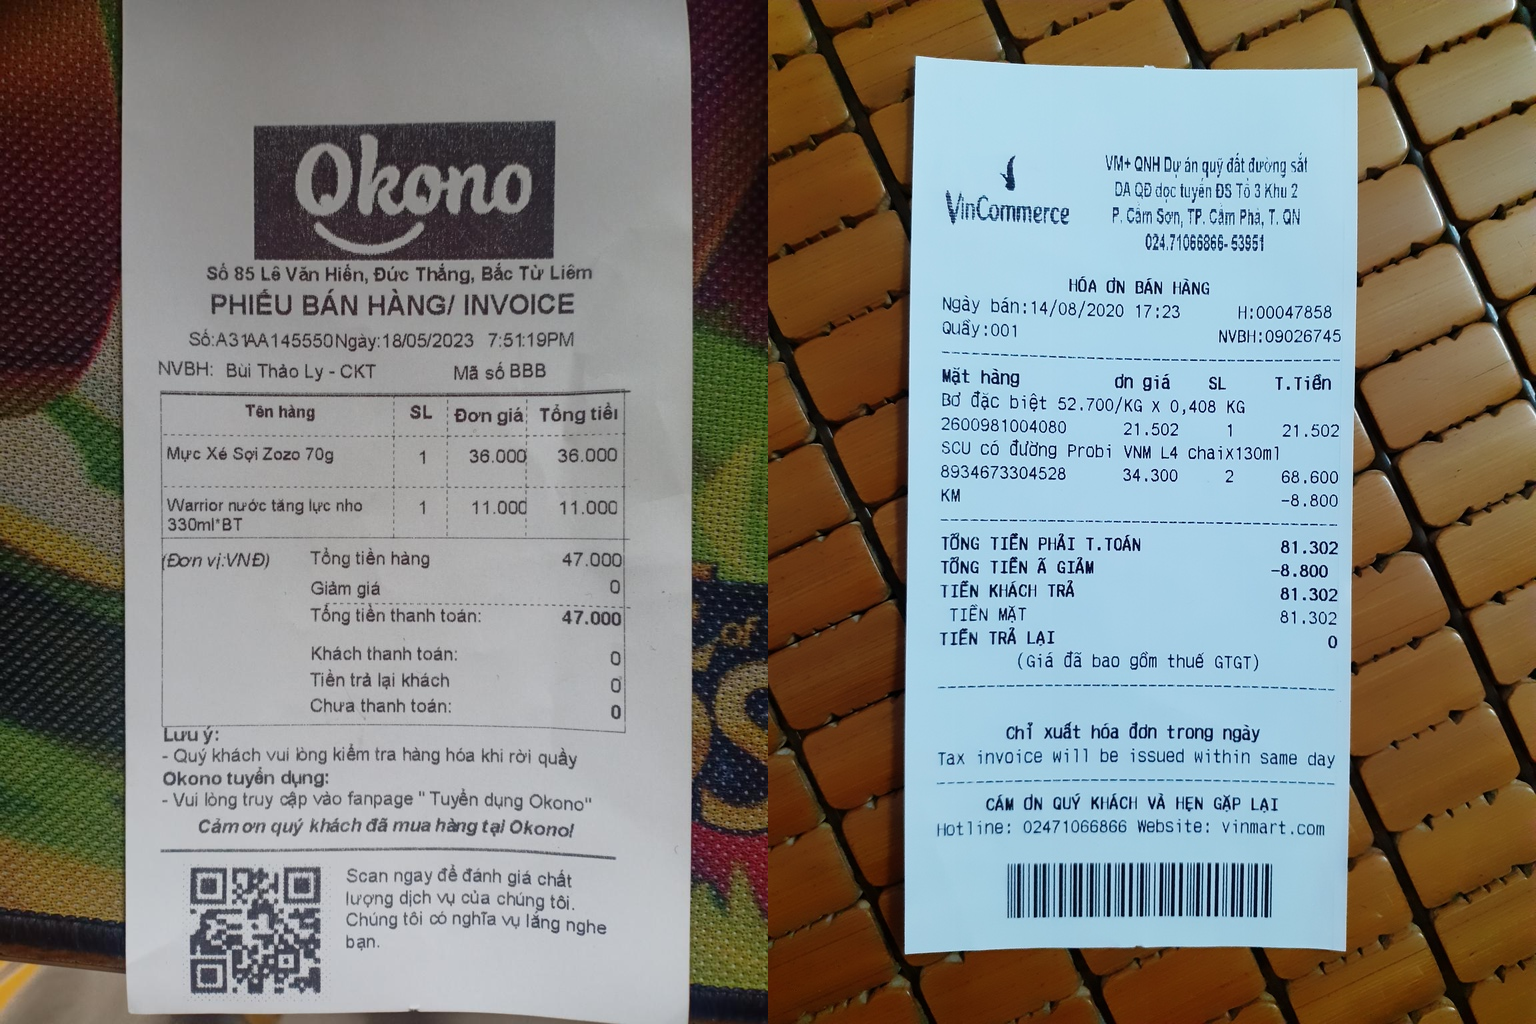
\includegraphics[scale=0.20]{images/okono-vincom.png}
    \centering
    \caption{Hóa đơn Okono(trái) và VinCommerce(phải)}
    \label{fig9-okono-vincom}
\end{figure}

Qua việc tập trung vào loại hóa đơn bán hàng cửa hàng tiện lợi và siêu thị, mong muốn thực hiện một nghiên cứu chi tiết về cách ứng dụng công nghệ OCR vào việc nhận dạng và xử lý dữ liệu từ hóa đơn trong ngữ cảnh thực tế.

\subsection{Chuẩn bị dữ liệu}
Chuẩn bị dữ liệu đây là một bước quan trọng để đảm bảo rằng mô hình OCR hoạt động tốt trên các dữ liệu thực tế. Trong phần này, em sẽ trình bày quá trình chuẩn bị và xử lý dữ liệu hình ảnh của hóa đơn. Tùy với nhiệm vụ khác nhau trong OCR ta có cách chuẩn bị dữ liệu khác nhau. Để thực hiện gán nhãn dữ liệu OCR, em sử dụng công cụ PPOCRLabel. Dưới đây là các bước thực hiện:

\textbf{Bước 1}: Chuẩn bị tập dữ liệu cần gãn nhãn
Ở bước này em chuẩn bị hơn 75 ảnh hóa đơn của cửa hàng tiện lợi Okono và xác định số lớp cần gãn nhãn cho bài toán KIE.  

\textbf{Bước 2}: Chạy chương trình PPOCRLabel
\begin{lstlisting}[language=bash]
    PPOCRLabel --kie True # [KIE mode] for [detection + recognition + keyword extraction] labeling
\end{lstlisting}
\begin{figure}[h]
    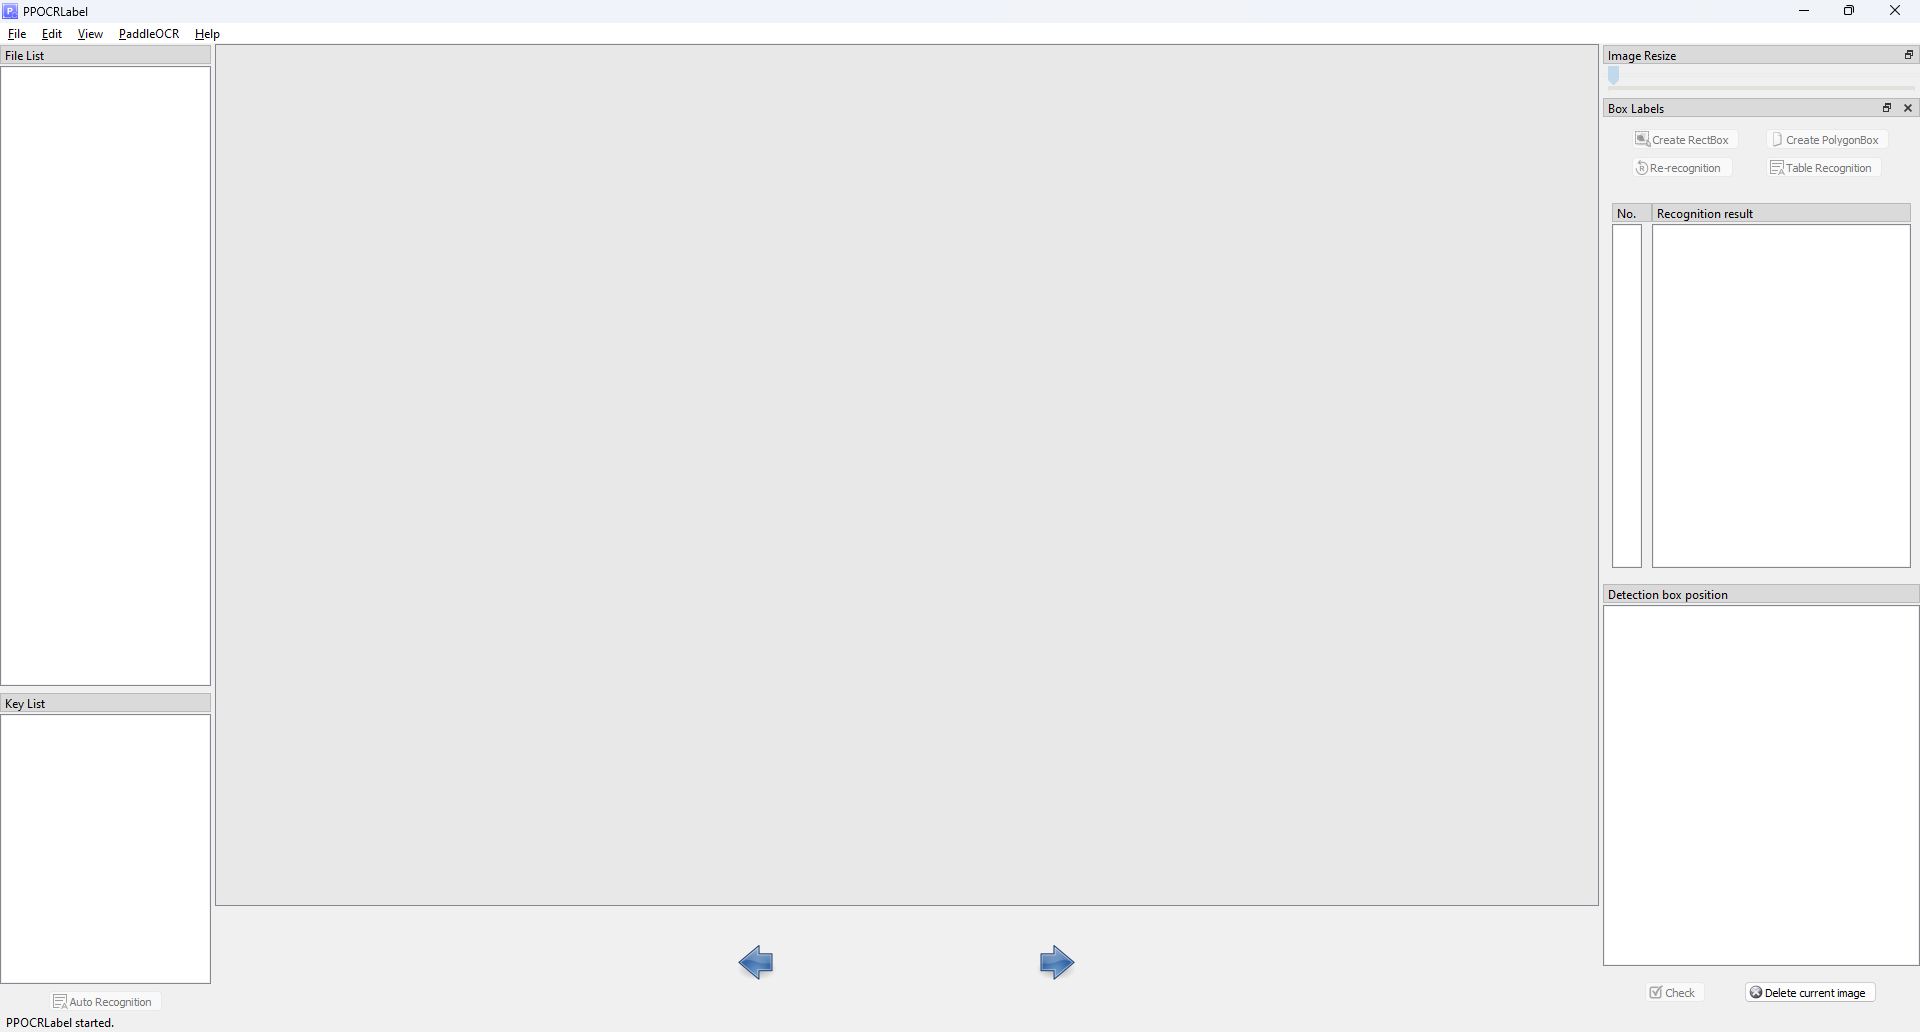
\includegraphics[scale=0.25]{images/UI-ppocr.png}
    \centering
    \caption{Giao diện PPOCRLabel}
\end{figure}

\textbf{Bước 3}: Nhấp vào nút "Open Dir" để mở thư mục chứa các hình ảnh cần gán nhãn. Các hình ảnh sẽ hiển thị trong danh sách.
\begin{figure}[h]
    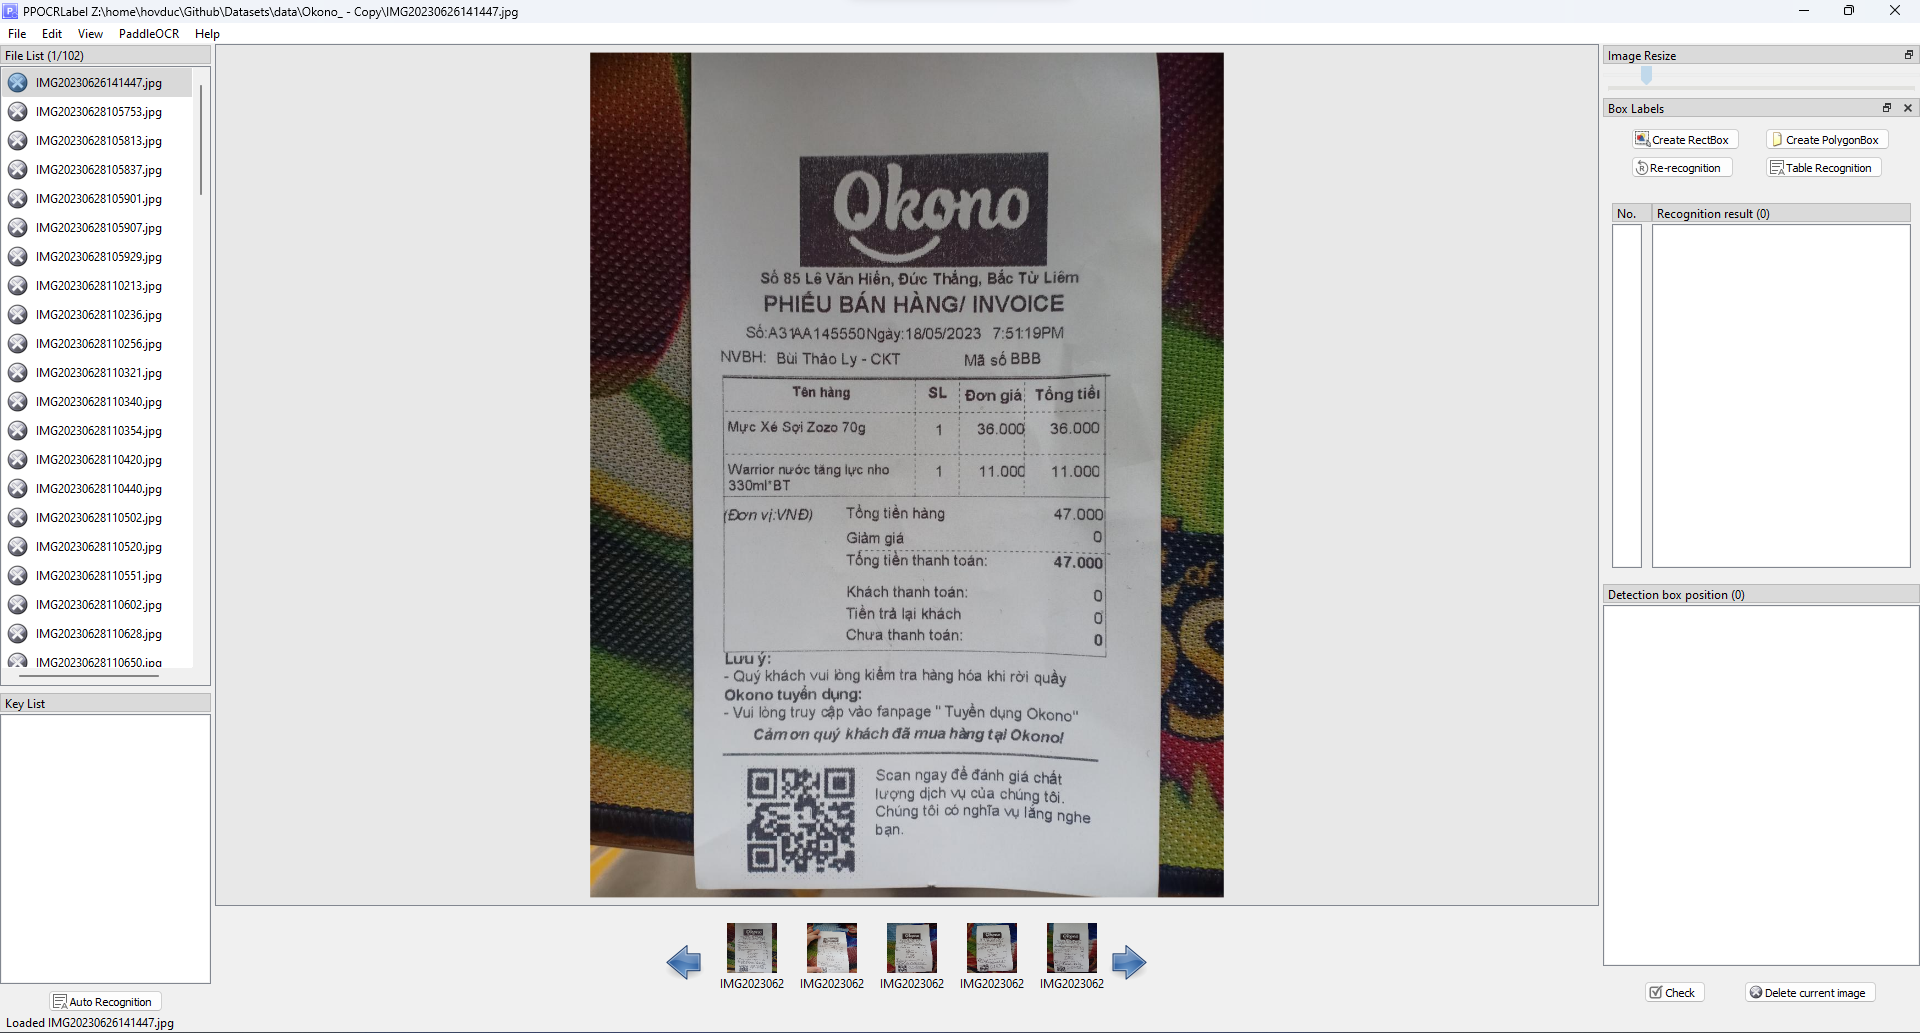
\includegraphics[scale=0.25]{images/UI-ppocr-image.png}
    \centering
    \caption{Danh sách ảnh PPOCRLabel}
\end{figure}

\textbf{Bước 4}: Chọn một hình ảnh, sử dụng các công cụ vẽ để khoanh vùng văn bản và gán nhãn tương ứng. Có thể gán nhiều vùng văn bản cho một hình ảnh.
\begin{itemize}
    \item W: để tạo một hộp cho phát hiện văn bản.
    \item Ctrl + E: Sửa nhãn của hộp.
    \item Ctrl + X: Thay đổi lớp của nhãn dùng cho gãn nhãn KIE.
\end{itemize}
Ở đây số lớp của bài toán KIE em xác định bao gồm các lớp sau:
\begin{itemize}
    \item OTHER: 
    \item SELLER: Tên cửa hàng
    \item ADDRESS: Địa chỉ 
    \item TIMESTAMP: Thời gian mua
    \item STAFF: Nhân viên bán hàng
    \item PRODUCT: Sản phẩm đã mua
    \item NUMBER: Số lượng sản phẩm
    \item PRICE: Giá của sản phẩm
    \item TOTAL\_COST: Tổng tiền thanh toán
\end{itemize}
\begin{figure}[h]
    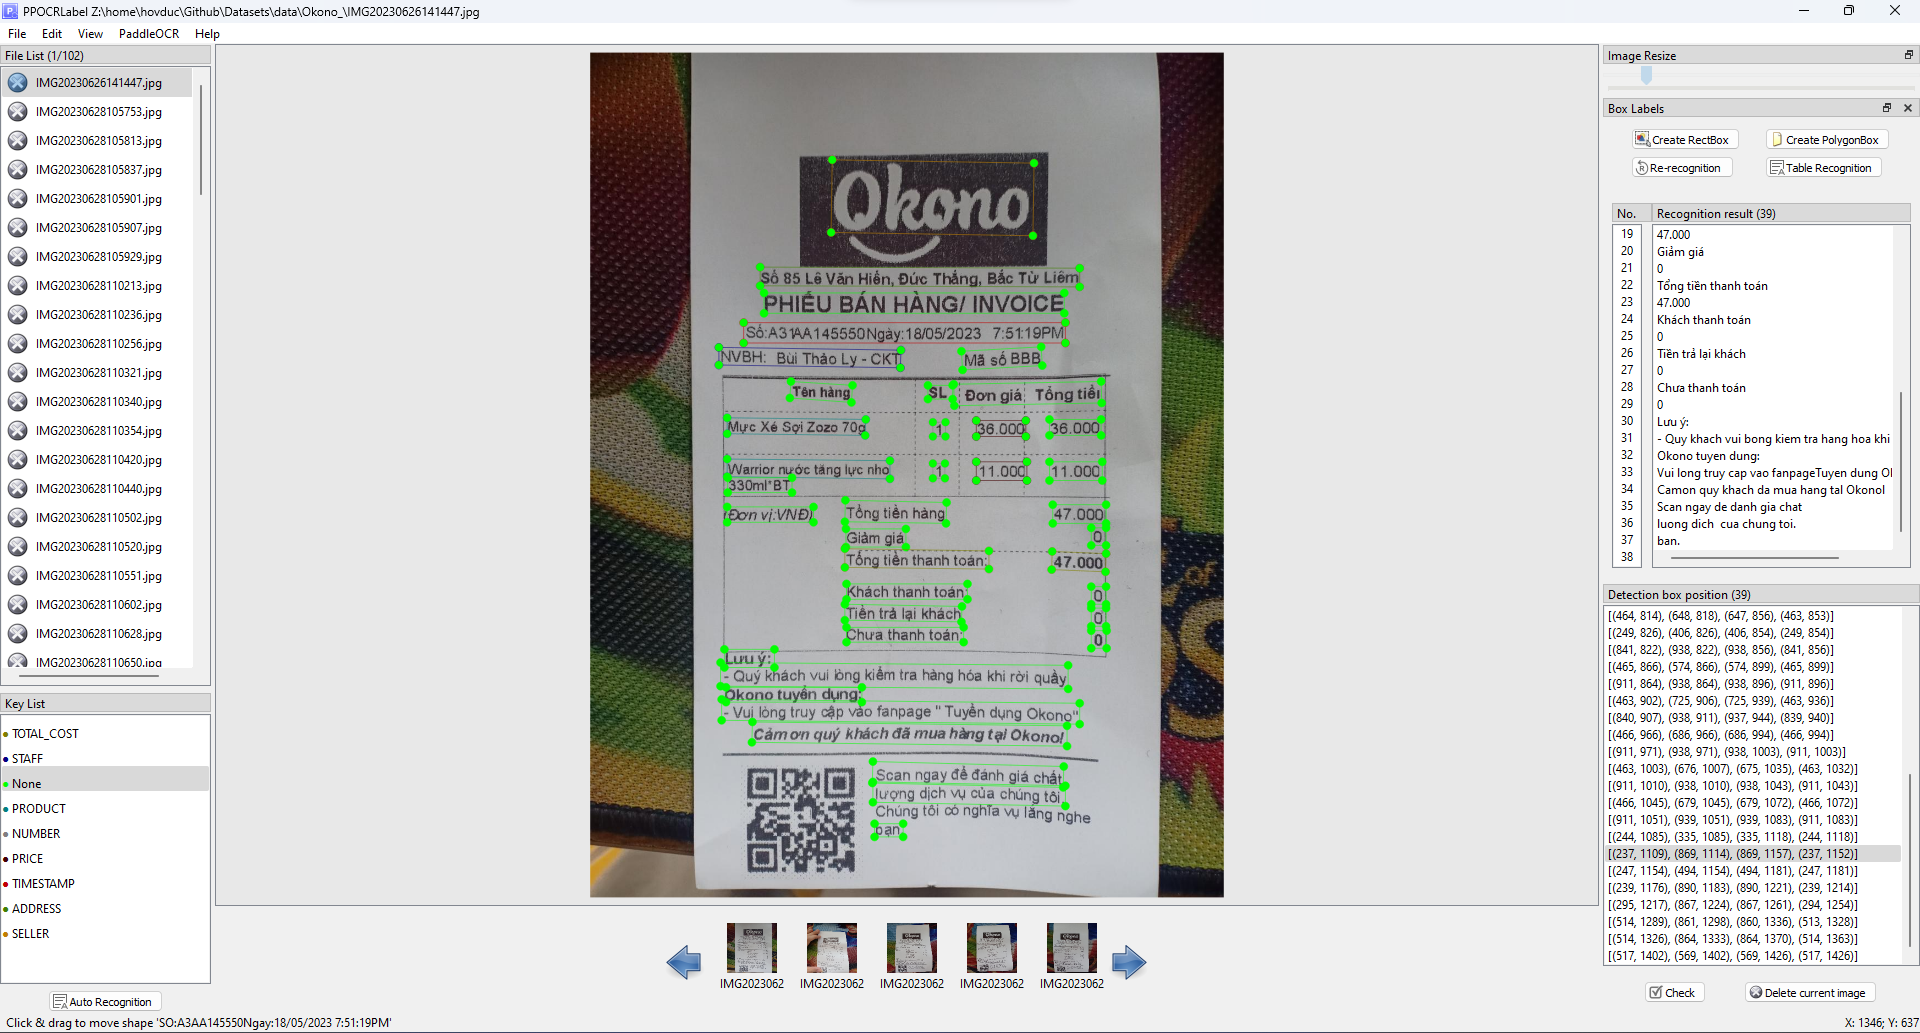
\includegraphics[scale=0.25]{images/GUI-ppocr-labeled.png}
    \centering
    \caption{Gán nhãn ảnh với PPOCRLabel}
\end{figure}

\textbf{Bước 5}: Lưu các thay đổi bằng nút "Save" hoặc tự động lưu khi thoát chương trình.

\textbf{Bước 6}: Tiếp tục gán nhãn cho các hình ảnh còn lại.

\textbf{Bước 7}: Nhấn nút "Export Recognition Result" để cắt ảnh cho tác vụ training nhận dạng văn bản.
\begin{figure}[h]
    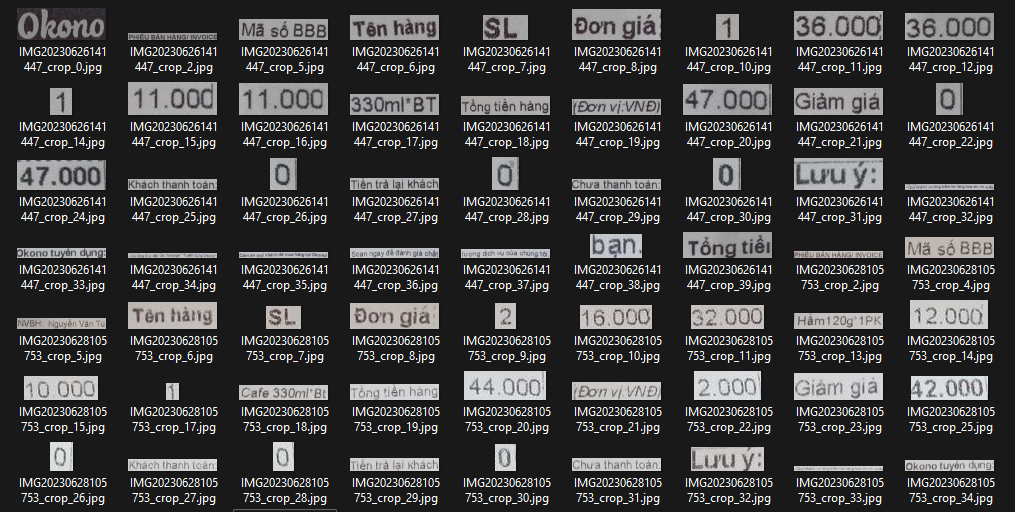
\includegraphics[scale=0.45]{images/data-invoice-text-recognition.png}
    \centering
    \caption{Dữ liệu hóa đơn được export từ PPOCRLabel}
\end{figure}

\textbf{Bước 8}: Kết thúc trương trình

Sau khi gãn nhãn xong ta thu được một file Label.txt, file có format như sau: 
\begin{lstlisting}[language=bash]
    image_files/IMG20230626141447.jpg	[{"transcription": "Okono", "points": [[440, 195], [807, 201], [805, 333], [438, 327]], "difficult": false, "key_cls": "SELLER"}...]
    image_files/IMG20230628105753.jpg	[{"transcription": "Okono", "points": [[429, 469], [700, 469], [700, 542], [429, 542]], "difficult": true, "key_cls": "SELLER"}...]
\end{lstlisting}

Các điểm trong các từ điển đó biểu thị tọa độ $(x, y)$ của bốn điểm của hộp văn bản, được sắp xếp theo chiều kim đồng hồ từ điểm ở góc trên bên trái. Trong transcription đại diện cho văn bản trong hộp, và key\_cls đại diện cho lớp của văn bản.

Dữ liệu cho nhận dạng văn bản khi export từ PPOCRLabel có format như sau:
\begin{lstlisting}[language=bash]
    #Tên ảnh                      #Thông tin chú thích ảnh
    IMG20230626141447_crop_0.jpg	Okono
    IMG20230626141447_crop_2.jpg	PHIẾU BÁN HÀNG/ INVOICE
    IMG20230626141447_crop_5.jpg	Mã số BBB
    IMG20230626141447_crop_6.jpg	Tên hàng
    IMG20230626141447_crop_7.jpg	SL
    ...
\end{lstlisting}
Để cho đúng dữ liệu cho bài toán này ta cần đưa nó về chuẩn LMDB:

\subsection{Tổng quan về dữ liệu đào tạo}
Dữ liệu cho nhiệm vụ phát hiện văn bản và KIE có cấu trúc như sau:
\begin{lstlisting}[language=bash]
|-train_data
    |- invoice
        |- train
            |- image_files
                |- image_001.jpg
                |- image_002.jpg
                | ...
            | train.txt
        |- valid
            |- image_files
                |- image_001.jpg
                |- image_002.jpg
                | ...
            | valid.txt  
\end{lstlisting}

Bao gồm 
Dữ liệu cho nhiệm vụ phát hiện văn bản và KIE có cấu trúc như sau:
\begin{lstlisting}[language=bash]
    |-train_data
        |- invoice-rec
            |- images
                |- image_001.jpg
                |- image_002.jpg
                | ...
            |- train.txt
            |- valid.txt
    \end{lstlisting}

\section{Huấn luyện mô hình}
Để huấn luyện mô hình OCR cho nhiệm vụ nhận diện hóa đơn đây là một quá trình phức tạp đòi hỏi sự kết hợp giữa nhiều nhiệm vụ khác nhau, mỗi nhiệm vụ là một quá trình huấn luyện riêng biệt. Điều này đảm bảo chất lượng của quá trình nhận dạng như Phát hiện vùng văn bản, Nhận dạng văn bản và Hiểu tài liệu(Document Understanding).

\subsection{Phát hiện văn bản}
Ở tác vụ này em lựa chọn thuật toán DBNet để phát hiện vùng văn bản. Sau khi quyết định được mô hình, download pre-trained model đã được train sẵn với dataset tiếng anh là ICDAR2015 dataset. Với backbone là ResNet50\_vd
\begin{lstlisting}[language=bash]
    # download the pre-trained model ResNet50_vd
    wget -P ./pretrain_models/ https://paddleocr.bj.bcebos.com/pretrained/ResNet50_vd_ssld_pretrained.pdparams
\end{lstlisting}

Bắt đầu training 
\begin{lstlisting}[language=bash]
python3 tools/train.py -c configs/det/det_r50_vd_db.yml  -o \
    Global.pretrained_model='./pretrain_models/ResNet50_vd_ssld_pretrained.pdparams' \
    Train.dataset.data_dir='./train_data/Okono_3/train/image/' \
    Train.dataset.label_file_list=['./train_data/Okono_3/train/train.txt'] \
    Train.loader.batch_size_per_card=12 \
    Eval.dataset.data_dir='./train_data/Okono_3/valid/image/' \
    Eval.dataset.label_file_list=['./train_data/Okono_3/valid/valid.txt'] \
    Global.save_model_dir='../drive/MyDrive/save/' \
    Global.checkpoints='/content/PaddleOCR/output/det_r50_vd' \
    Global.eval_batch_step=100 \
    Global.cal_metric_during_train=True \
\end{lstlisting}
\begin{lstlisting}[language=bash]
[2023/08/25 11:14:07] ppocr INFO: Architecture : 
[2023/08/25 11:14:07] ppocr INFO:     Backbone : 
[2023/08/25 11:14:07] ppocr INFO:         layers : 50
[2023/08/25 11:14:07] ppocr INFO:         name : ResNet_vd
[2023/08/25 11:14:07] ppocr INFO:     Head : 
[2023/08/25 11:14:07] ppocr INFO:         k : 50
[2023/08/25 11:14:07] ppocr INFO:         name : DBHead
[2023/08/25 11:14:07] ppocr INFO:     Neck : 
[2023/08/25 11:14:07] ppocr INFO:         name : DBFPN
[2023/08/25 11:14:07] ppocr INFO:         out_channels : 256
[2023/08/25 11:14:07] ppocr INFO:     Transform : None
[2023/08/25 11:14:07] ppocr INFO:     algorithm : DB
[2023/08/25 11:14:07] ppocr INFO:     model_type : det
...
eval model:: 100% 31/31 [00:03<00:00,  2.97it/s]
[2023/08/25 13:22:35] ppocr INFO: cur metric, precision: 0.2653061224489796, recall: 0.17067833698030635, hmean: 0.20772303595206393, fps: 14.512030517908638
[2023/08/25 13:22:35] ppocr INFO: best metric, hmean: 0.8958, is_float16: False, start_epoch: 156, precision: 0.9292, recall: 0.8648, fps: 13.95, best_epoch: 280
\end{lstlisting}

\subsection{Phát hiện văn bản}
Với tác vụ nhận dạng văn bản em sử dụng VietOCR. Dưới đây là các bước huấn luyện mô hình:
\begin{lstlisting}[language=Python]
    from vietocr.tool.config import Cfg
    from vietocr.model.trainer import Trainer
\end{lstlisting}

Load config VGG19 + Transformer và điều chỉnh tham số:
\begin{lstlisting}[language=Python]
    config = Cfg.load_config_from_name('vgg_transformer')
    dataset_params = {
        'name':'hw',
        'data_root':'./train_data/invoice-rec/',
        'train_annotation':'train.txt',
        'valid_annotation':'valid.txt'
    }

    params = {
            'print_every':200,
            'valid_every':15*200,
            'iters':20000,
            'checkpoint':'./checkpoint/transformerocr_checkpoint.pth',    
            'export':'./weights/transformerocr.pth',
            'metrics': 10000
            }

    config['trainer'].update(params)
    config['dataset'].update(dataset_params)
    config['device'] = 'cuda:0'
\end{lstlisting}

Bắt đầu huấn luyện mô hình:
\begin{lstlisting}[language=Python]
    trainer.train()
\end{lstlisting}

\begin{lstlisting}[language=Python]
iter: 000200 - train loss: 2.627 - lr: 1.51e-05 - load time: 0.72 - gpu time: 97.80
iter: 000400 - train loss: 2.367 - lr: 2.45e-05 - load time: 0.06 - gpu time: 91.02
iter: 000600 - train loss: 2.212 - lr: 3.95e-05 - load time: 0.07 - gpu time: 93.54
...
iter: 029600 - train loss: 0.526 - lr: 1.63e-07 - load time: 0.06 - gpu time: 84.60
iter: 029800 - train loss: 0.541 - lr: 4.14e-08 - load time: 0.06 - gpu time: 90.35
iter: 030000 - train loss: 0.550 - lr: 1.20e-09 - load time: 0.07 - gpu time: 90.14
iter: 030000 - valid loss: 0.551 - acc full seq: 0.8101 - acc per char: 0.9543
\end{lstlisting}

\subsection{Key information extraction}
Cuối cùng là mô hình KIE, ở đây em sử dụng LayoutXLM SER để huấn luyện. Dưới đây là các bước:

Download pretrained model và giải nén.
\begin{lstlisting}[language=bash]
    mkdir pretrained_model
    cd pretrained_model
    wget https://paddleocr.bj.bcebos.com/ppstructure/models/vi_layoutxlm/ser_vi_layoutxlm_xfund_pretrained.tar
    tar -xf ser_vi_layoutxlm_xfund_pretrained.tar
\end{lstlisting}

Bắt đầu huấn luyện mô hình:
\begin{lstlisting}[language=bash]
python tools/train.py -c ./configs/kie/vi_layoutxlm/ser_vi_layoutxlm_xfund_zh.yml -o \
    Architecture.Backbone=&num_classes \
    Train.dataset.data_dir=train_data/invoice/train/image_files \
    Eval.datasetdata_dir=train_data/invoice/valid/image_files \
    PostProcess.class_path=train_data/invoice/class_list.txt
\end{lstlisting}

\begin{lstlisting}[language=bash]
[2023/08/14 17:40:07] ppocr INFO: Architecture : 
[2023/08/14 17:40:07] ppocr INFO:     Backbone : 
[2023/08/14 17:40:07] ppocr INFO:         checkpoints : None
[2023/08/14 17:40:07] ppocr INFO:         mode : vi
[2023/08/14 17:40:07] ppocr INFO:         name : LayoutXLMForSer
[2023/08/14 17:40:07] ppocr INFO:         num_classes : 17
[2023/08/14 17:40:07] ppocr INFO:         pretrained : True
[2023/08/14 17:40:07] ppocr INFO:     Transform : None
[2023/08/14 17:40:07] ppocr INFO:     algorithm : LayoutXLM
[2023/08/14 17:40:07] ppocr INFO:     model_type : kie
...
[2023/08/14 19:05:50] ppocr INFO: cur metric, precision: 0.9857, recall: 0.9928, hmean: 0.9892, fps: 24
[2023/08/14 19:08:10] ppocr INFO: save best model is to ./output/ser_vi_layoutxlm_xfund_zh/best_accuracy
[2023/08/14 19:08:10] ppocr INFO: best metric, hmean: 0.9857, precision: 0.9928, recall: 0.9892, fps: 24, best_epoch: 57
\end{lstlisting}

\section{Kết quả mô hình}
\begin{table}[h]
    \centering
    \begin{tabular}{ | c | c | c | c | c | c | } 
        \hline
        \textbf{Task} & \textbf{Model} & \textbf{Backbone} & \textbf{Hmean} & \textbf{Precision} & \textbf{Recall} \\ 
        \hline
        Detection & DBNet & ResNet50vd & $89.58\%$ & $92.92\%$ & $86.48\%$ \\ 
        \hline
        KIE & LayoutXLM & LayoutXLM & $98.57\%$ & $99.28\%$ & $98.92\%$ \\ 
        \hline
        \hline
        \textbf{Task} & \textbf{Model} & \textbf{Backbone} & \textbf{Accuracy} & \multicolumn{2}{c|}{\textbf{Accuracy char}}   \\ 
        \hline
        Recognition & VietOCR & VGG19 & $81.01\%$ & \multicolumn{2}{c|}{$95.43\%$} \\ 
        \hline
    \end{tabular}
    \caption{Độ chính xác của cả 3 mô hình}
    \label{table:1}
\end{table}

Kết quả huấn luyện của mô hình đạt được đều thu được kết quả tốt, đặc biệt là với mô hình \acrshort*{kie} cho ra độ chính xác cao nhất (Bảng \ref{table:1}). Tuy vậy ở tác vụ nhận dạng văn bản độ chính xác của mô hình trên toàn bộ chuỗi chỉ đạt $81.01\%$, điều này ảnh hưởng không ít đến thông tin được lưu trữ của đề tài.

Trong chương \ref{data_train}, em đã mô tả xong loại hóa đơn dùng cho đồ án, quá trình thu thập và xử lý dữ liệu, các bước huấn luyện mô hình và kết quả huấn luyện của từng mô hình. Ở chương tiếp theo của báo cáo, em sẽ mô tả quá trình xây dựng chương trình hoàn chỉnh và trình bày các kết quả của chương trình.
